\section{Applications of convolution}

This chapter only scratches the practical and theoretical uses of
convolution and linear time-invariant systems. I'll use two examples
to illustrate the application of a one-dimensional convolution
equation. Be aware that these are by no means the only types of
situations where you will encounter a convolution. Chances are quite
high that a signal processing system you can think of is an LTI
system, or can be approximated as one. Convolution can be found
everywhere!

\subsection{Example: Radar and sonar equation}

\begin{marginfigure}
\begin{center}
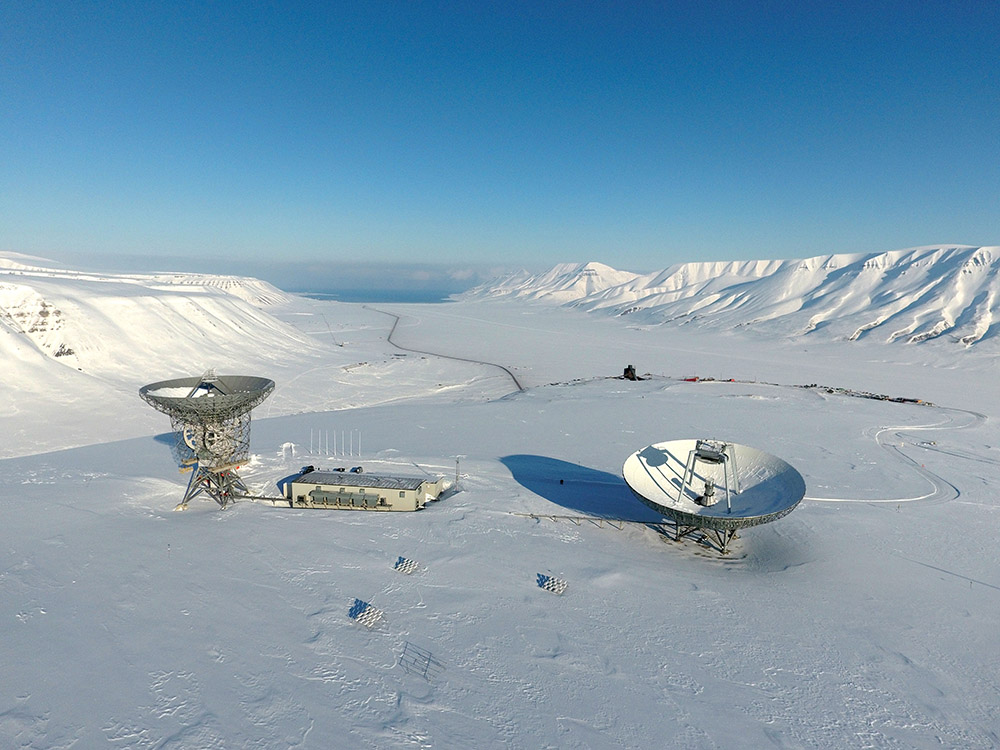
\includegraphics[width=\textwidth]{Applications/figures/svalbard.jpg}
\end{center}
\caption{EISCAT Svalbard Radar. The radar echo from the D-region of the ionosphere can be modeled using the equation shown in Equation \ref{eq:convolution_radar}. Photo: Craig Heinselman}
\label{fig:eiscat_svalbard}
\end{marginfigure}
The convolution equation is often used to model radar and sonar
measurements. In this case, the impulse response signal $h[n]$
represents the signal that is scattered as a function of distance. The
signal $x[n]$ represents what a radar or sonar transmits. The signal
received by a radar or sonar receiver $m[n]$ is then modeled as:
\begin{align}
m[n] &=  h[n]*x[n]\\
     &= \sum_{r=0}^{M} h[r] x[n-r]. \label{eq:convolution_radar}\,\,.
\end{align}
In this case, the index $r \in \mathbb{N}$ represents round-trip
propagation time between the transmitter and the receiver. The larger
the distance between the transmitter and the receiver, the larger the
delay. Assuming that the sample rate is $f_s$ in units of hertz or
($\frac{1}{\mathrm{s}}$), and the group velocity of the transmitter
wave $v_g$ ($\frac{\mathrm{m}}{\mathrm{s}}$), the round-trip range is given by:
\begin{equation}
R = \frac{v_g r}{2 f_s}\,\,.
\end{equation}
In the case of radar, the group velocity for electromagnetic waves is
$v_g \approx 3 \cdot 10^8$ ($\frac{\mathrm{m}}{\mathrm{s}}$). For sonar, it is the speed of
acoustic waves within the medium. In the case of air, this is
$v_g \approx 343$ ($\frac{\mathrm{m}}{\mathrm{s}}$).

To see how the convolution equation is the radar equation, we can use
an illustration, as shown in Figure \ref{fig:range_time_diagram}.
\begin{figure}
\begin{center}
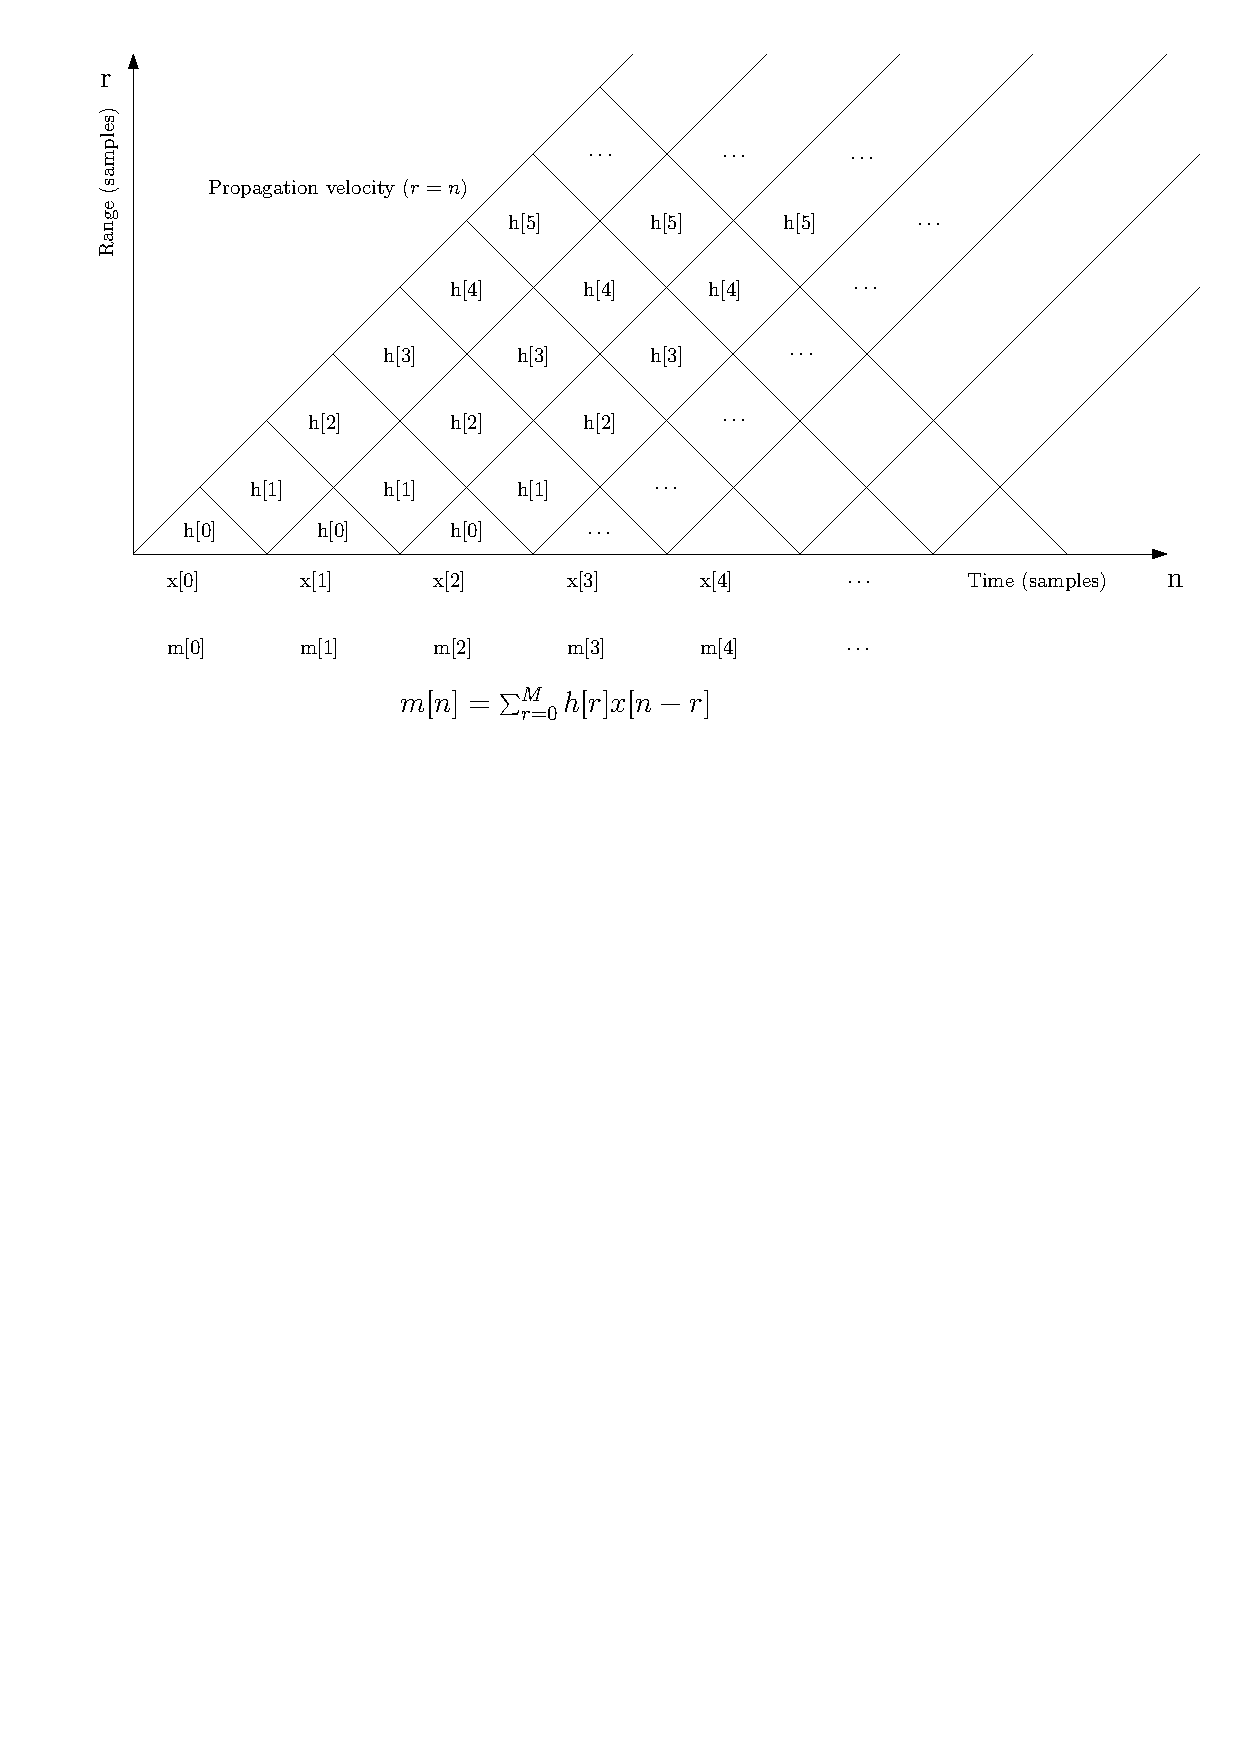
\includegraphics[width=\textwidth]{Applications/figures/rd.pdf}
\end{center}
\caption{A range-time diagram depicting the relationship between a transmitted signal and a scattered signal.}
\label{fig:range_time_diagram}
\end{figure}

If the probing signal is a unit impulse $x[n]=\delta[n]$ (a very short
radar pulse), then the measurement directly provides the scattering
amplitude as a function of range:
\begin{align}
m[n] = \sum_{r=0}^M h[r]\delta[n-r] = h[r]\,\,.
\end{align}
This type of radar is called a pulsed radar. In terms of radar
signal processing, this is the easiest case, as no signal processing
is needed! A radar measurement in this case is equivalent to measuring
the ``impulse response'' of the region that the radar is probing.

Here is a fascinating example of a blind child that has learned to
click his tongue (emitting a $\delta[n]$-like impulse sound) to probe the
acoustic scattering of his
surroundings \url{https://www.youtube.com/watch?v=fnH7AIwhpik}. While
this may seem like a superhuman feat, this is not unlike measuring the
distance between yourself and a mountain side by shouting ``echo''
very loudly and counting how long it takes for you to hear a strong
echo. I am sure that many of you have done this already.

\begin{marginfigure}
\begin{center}
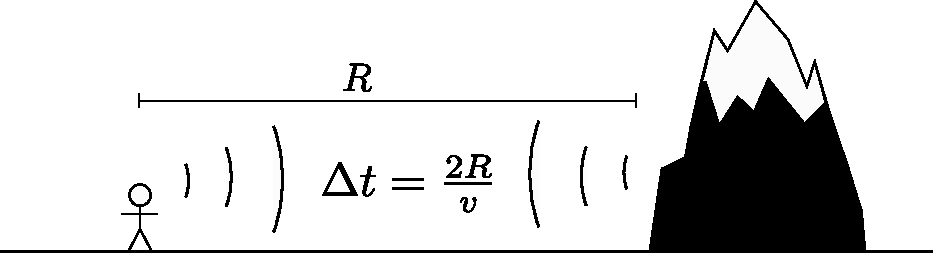
\includegraphics[width=\textwidth]{Applications/figures/mountain_echo.pdf}
\end{center}
\caption{The acoustics of a space are determined by acoustic waves
scattered from various obstacles at various propagation delays. This
can be quite precisely modeled using a convolution, assuming that
nothing is moving.}
\end{marginfigure}

If the transmitted waveform $x[n]$ is more complicated than a unit
impulse, the measurements need to be filtered in some way to
reconstruct the scattered signal as a function of range $h[n]$. This
is achieved by designing a filter $\lambda[n]$, which has the
following property $\lambda[n]*x[n] \approx \delta[n]$. After applying
the filter $\lambda[n]$ to the measured signal, one obtains the echo
as a function of range:
\begin{align}
\lambda[n]*m[n] = \lambda[n]*h[n]*x[n] = (\lambda[n]*x[n])*h[n]\approx h[n]\,\,. 
\end{align}
Design of pairs of signals $x[n]$ and filters $\lambda[n]$ is a topic
of radar signal processing. An example of a good pairing of a radar
transmit signal and a receiver filter is shown in the following convolution animation:
\url{http://kaira.uit.no/juha/fir_animation/ex12.gif}.
This is the so-called 13-bit Barker code and the inverse filter that
corresponds to it. The convolution of these two signals is the unit
impulse.